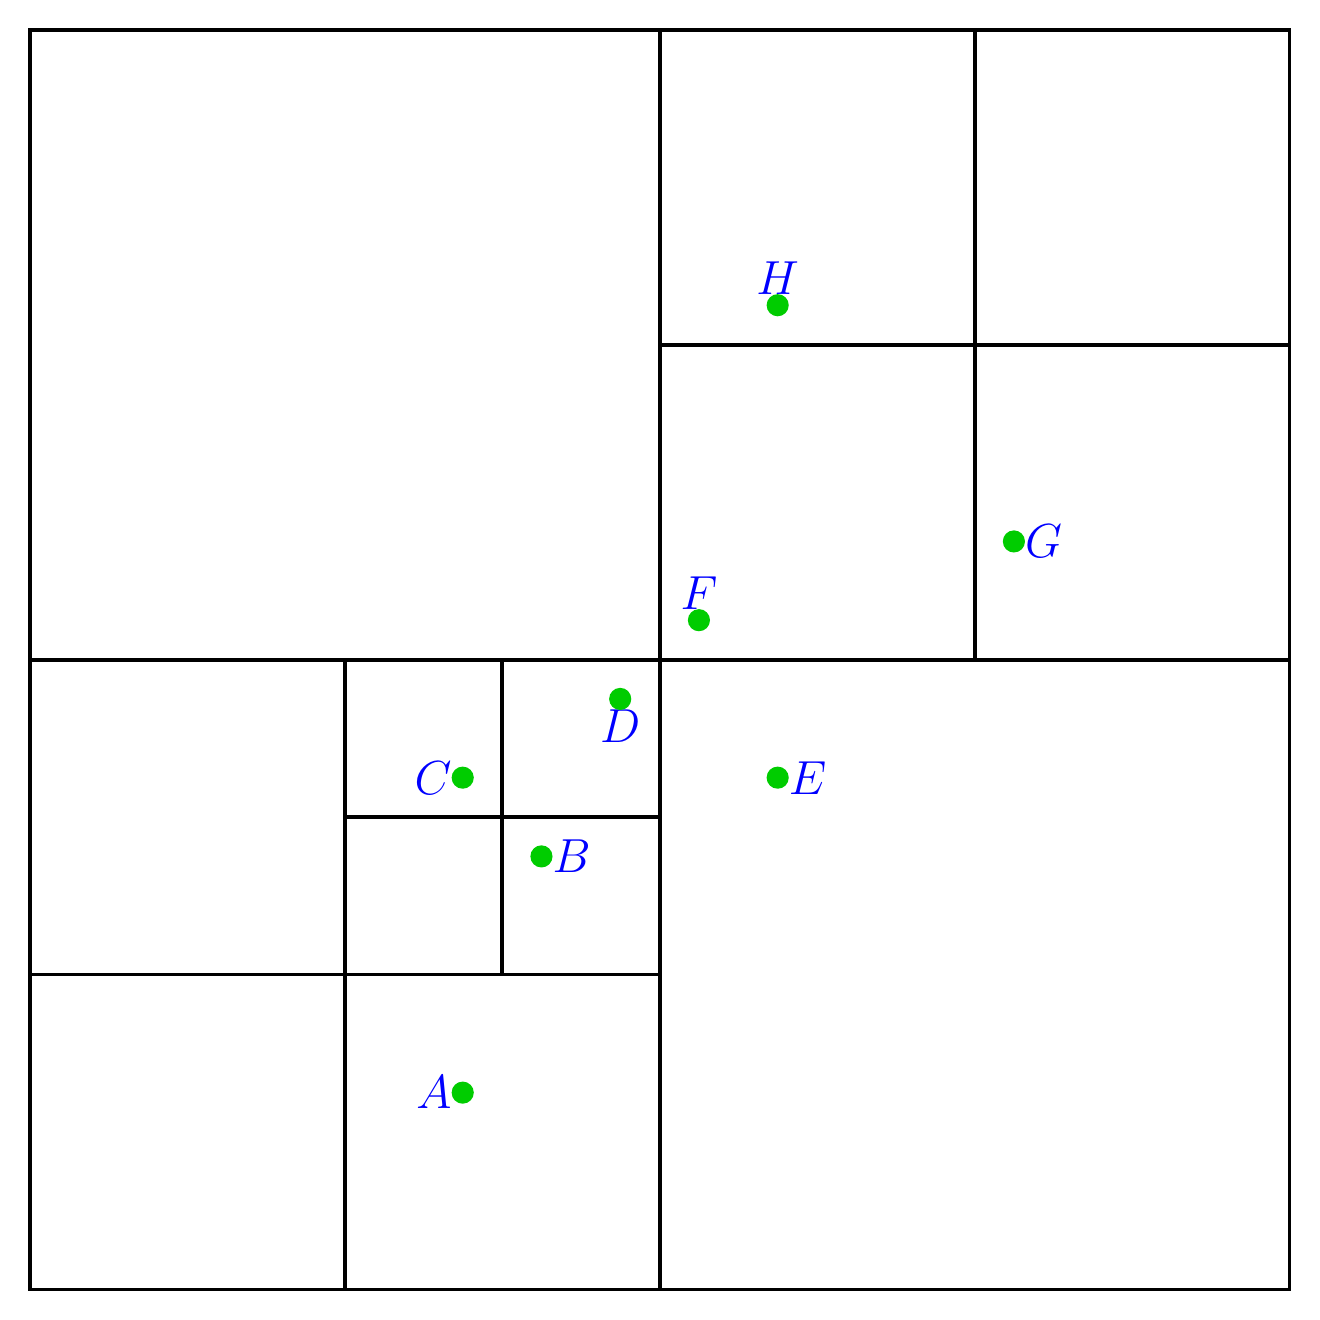
\begin{tikzpicture}[line width=.5mm]
    \def\A{\LARGE{\textcolor{blue}{$A$}}}
    \def\B{\LARGE{\textcolor{blue}{$B$}}}
    \def\C{\LARGE{\textcolor{blue}{$C$}}}
    \def\D{\LARGE{\textcolor{blue}{$D$}}}
    \def\E{\LARGE{\textcolor{blue}{$E$}}}
    \def\F{\LARGE{\textcolor{blue}{$F$}}}
    \def\G{\LARGE{\textcolor{blue}{$G$}}}
    \def\H{\LARGE{\textcolor{blue}{$H$}}}

    \draw (0, 0) rectangle (16, 16);

    \coordinate [label=left:\A] (A) at (5.5, 2.5);
    \coordinate [label=right:\B] (B) at (6.5, 5.5);
    \coordinate [label=left:\C] (C) at (5.5, 6.5);
    \coordinate [label=below:\D] (D) at (7.5, 7.5);
    \coordinate [label=right:\E] (E) at (9.5, 6.5);
    \coordinate [label=above:\F] (F) at (8.5, 8.5);
    \coordinate [label=right:\G] (G) at (12.5, 9.5);
    \coordinate [label=above:\H] (H) at (9.5, 12.5);

    \draw (8, 0) -- (8, 16);
    \draw (0, 8) -- (16, 8);
    \draw (4, 0) -- (4, 8);
    \draw (0, 4) -- (8, 4);
    \draw (4, 6) -- (8, 6);
    \draw (6, 4) -- (6, 8);
    \draw (8, 12) -- (16, 12);
    \draw (12, 8) -- (12, 16);

    \foreach \point in {A, B, C, D, E, F, G, H}
        \fill [green!80!black] (\point) circle (4pt);
\end{tikzpicture}

% vim: set ff=unix tw=79 sw=4 ts=4 et ic ai :
